\documentclass{../../text-style}

\texttitle{Лекция 8: Работа в команде}

\begin{document}

\maketitle
\thispagestyle{empty}

\attribution{Тимофей Александрович Брыксин, бывш. доцент кафедры системного программирования СПбГУ}

\section{Команда}

Команда~--- сплочённая группа людей, объединенная единой целью, но при этом результат, над которым ведется работа, не состоит только из частей, сделанных отдельно каждым участником: для объединения результатов работы отдельных членов команды требуется дополнительная работа. (Для сравнения: 10 разнорабочих на стройке, копающих ямы~--- не команда, поскольку они друг с другом не взаимодействуют. Если заменить одного из них на другого, никто не заметит перемен, а в командах так не работает).

Хорошая команда~--- не менее важная составляющая успешного проекта, чем планирование и т.п., скорее даже более важная, поскольку слабая, неслаженная команда не просто непродуктивна, но и может являться причиной, по которой отдельные люди могут выгорать, переживать большое количество стресса ежедневно, а то и вообще покинуть проект.

Команду составляют именно разработчики, поэтому при переходе в новую команду/создании своей разработчику нужно понимать, куда он попадает. Команда~--- источник существенной части удовлетворения от работы. Можно делать плохие проекты в хорошей команде и быть счастливым, но даже делать хорошие проекты в плохой команде будет не так весело.

С командой разработчик проводит в среднем восемь часов в день, поэтому от того, насколько хорошо устроены процессы в команде, зависит очень многое. Исходя из этого, очень важно понимать состояние и общее настроение команды, особенно если что-то идёт не так. Если в команде что-то идёт не так, необходимо задуматься о том, как это можно исправить. По этим причинам создать высокоэффективную команду очень сложно.

Для проверки сплоченности команды нужно убедиться в том, что:

\begin{itemize}
    \item члены команды взаимодействуют друг с другом с целью выполнения своих заданий;
    \item команда производит цельный проект/продукт/сервис/..., а не просто отдельные компоненты.
\end{itemize}

Грамотный менеджер будет пытаться сделать так, чтобы каждый член команды ощущал некоторую причастность к команде и проекту в целом, чтобы проект стал для разработчиков <<своим>>. Практика показывает, что если люди ассоциируют себя с проектом, то вкладываются в работу лучше. Ну и конечно же грамотный менеджер будет пытаться строить комфортную и позитивную атмосферу: счастливый разработчик~--- почти всегда продуктивный разработчик.

Но создать такую команду очень сложно по ряду причин. Может показаться, что сплоченность, эффективность команды~--- дело удачи, совпадения характеров людей. Однако эти факторы слишком важны для продуктивной работы, чтобы доверить их удаче. Поэтому выделим два фактора, которые должны быть соблюдены для того, чтобы команда была действительно высокоэффективной. Во-первых, нужно понимать, что команда формируется для того, чтобы решать сложные проблемы, и решать их вместе. Во-вторых, члены команды разные, и поэтому они должны научиться работать вместе. И если первый пункт довольно очевиден, то второй рассмотрим более подробно.

Как же сделать так, чтобы абсолютно разные люди хорошо работали вместе? Во-первых, не существует двух людей с абсолютно одинаковым уровнем. Более того (обычно характерно для новичков в профессии), люди могут попросту не уметь работать в команде. Поэтому из разработчиков нужно сделать команду, которая будет двигаться вместе. Нужно понимать, что по сути проект~--- это набор задач, которые нужно решить, и у всех людей очень разный подход к решению поставленных задач. Как правило, это может быть очень разный профессиональный уровень, разная продуктивность, подходы к общению, разный темперамент. Кто-то мыслит более глобально, кто-то больше вдается в детали. Кроме того, не стоит исключать человеческий фактор: люди могут банально ненавидеть друг друга просто так (или, напротив, относиться друг к другу слишком хорошо). Таких разных людей очень сложно заставить слаженно работать вместе, поскольку они не смогут продуктивно взаимодействовать друг с другом. Нужно понимать, что если члены команды сами не захотят учиться быть частью команды, то с этим вряд ли удастся что-то сделать, проще просто найти другого человека. Но если человек готов меняться, проводить самоанализ, становиться <<более гибким>>, то есть шанс, что применение определенных практик по введению этого человека в команду принесёт определенный успех.

На картинке ниже можно увидеть своеобразную метафору: есть точка A, есть точка B, а мы с помощью команды пытаемся перейти по мосту, состоящему из разных умений/навыков, в точку B из точки A. Следует иметь в виду, что мост разрушится, если что-то не будет работать так, как должно. Кроме того, можно провести аналогию с архитектурой: высокоэффективная команда требует наличия каждой составляющей, изображенной на картинке; суть архитектуры заключается в том, как индивидуальные составляющие работают вместе; недостаток в одном компоненте не может быть компенсирован другим компонентом.

\begin{center}
    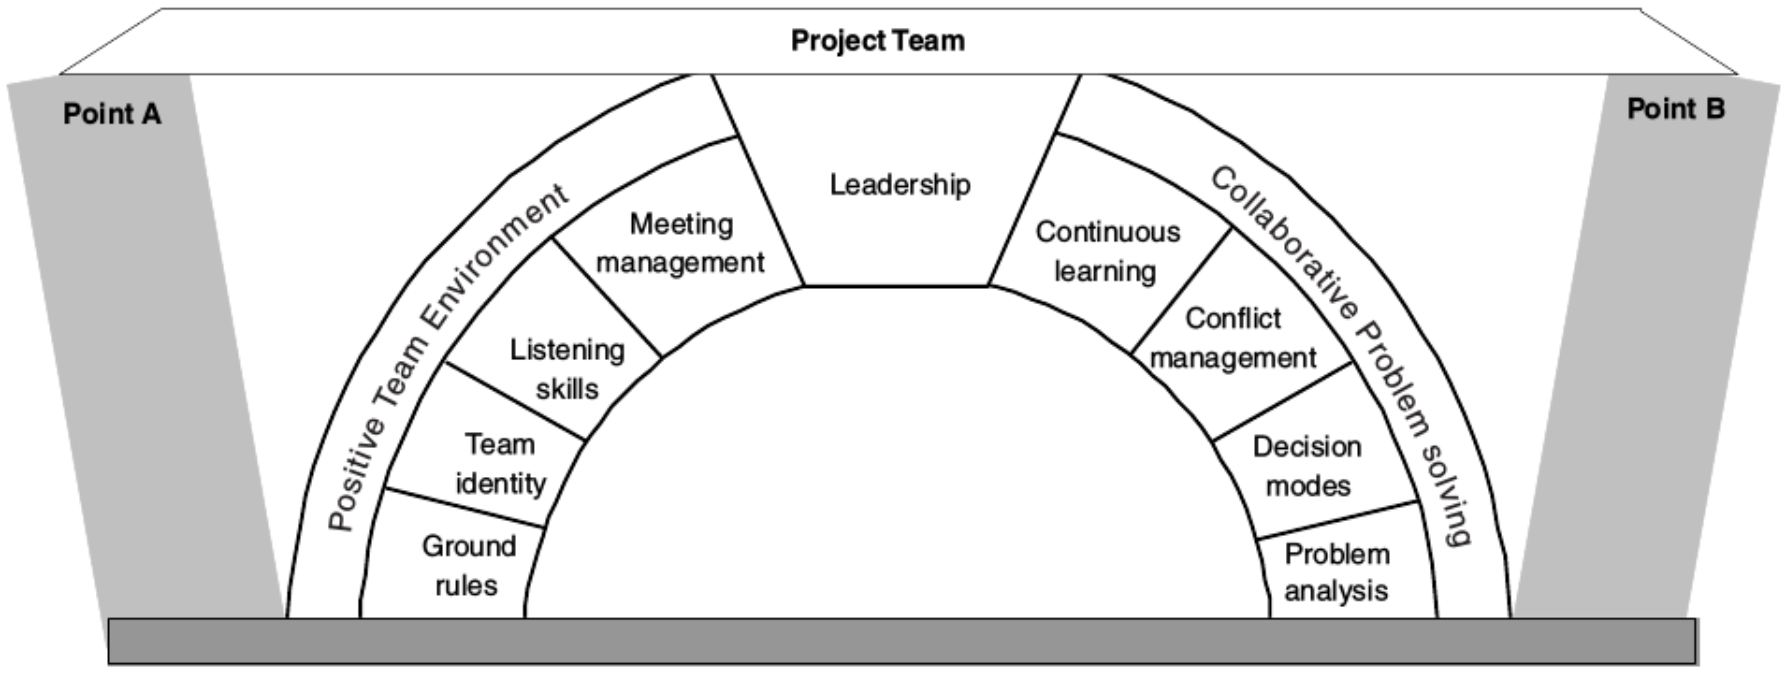
\includegraphics[width=0.95\textwidth]{successfulTeamComponents.png}
\end{center}

На схеме выделяются три основных области: позитивная экосистема команды, лидерство и совместное решение проблем. Не будем подробно рассматривать лидерство, но отметим, что если у руководителя команды нет лидерских качеств, то ему будет сложно вести за собой других людей. Две другие компоненты рассмотрим более подробно.

\section{Позитивная экосистема команды}

Когда люди приходят на работу, они не хотят превозмогать сложности, они хотят прийти, попасть в комфортную обстановку и начать работать. Разумеется, всё это должно быть в разумных пределах. Не должно быть условий, способствующих излишней расслабленности членов команды, но и мысли в духе <<эх, ну ща начнется>> не должны посещать человека каждое утро, когда он приходит на работу. К такой экосистеме надо стремиться, поскольку она позволяет достичь доверия в коллективе, взаимоуважения и настоящей эффективности.

Рассмотрим теперь каждый из пунктов данной компоненты:

\paragraph*{Правила в команде.} Обычно их не фиксируют строго формально, но хотя бы неформально они должны быть известны всем. Они определяют ценности команды, правила поведения внутри коллектива. Это позволяет создать комфортную атмосферу внутри коллектива. Даже если эти правила не сформулированы явным образом, их всё же стоит понимать, и за ними нужно следить.

\paragraph*{Сплоченность команды.} Перед командой должна быть поставлена единая общая цель. Люди имеют  определенные цели, и у каждого человека они свои: кто-то хочет учиться, кто-то общаться с интересными людьми, кто-то~--- просто заработать денег и т.д. Надо заставить этих людей двигаться к общей цели, которая ставится перед всем проектом.

\paragraph*{Умение слушать.} Если люди не умеют слушать друг друга, они ни о чем не договорятся, а взаимопонимания, взаимоуважения внутри команды просто не будет, как не будет и эффективности. Следует помнить, что нет задачи сделать людей друзьями, но им должно быть комфортно вместе. Человеку не будет комфортно среди людей, которые относятся к его идеям с пренебрежением.

\paragraph*{Умение организовывать совещания.} Команда пытается делать совместные действия на пути к общей цели, а это возможно только тогда, когда люди собираются вместе. Совещания должны проходить регулярно: например, раз в день или несколько дней. Культура проведения совещания должна быть определена, а если её нет, нужно её создать и воспитывать. Это ещё один ключ к высокой эффективности команды.

Даже после такого поверхностного анализа каждого из пунктов можно понять, что позитивная атмосфера в команде~--- это не абстрактная, а вполне конкретная вещь, а если быть точнее~--- набор умений, которыми менеджер проекта должен владеть сам и привить членам своей команды. Впоследствии всё это в целом ведёт к двум очень важным факторам высокой продуктивности команды:

\begin{itemize}
    \item персонализация командной цели: каждый член команды начинает расценивать свой успех в терминах общего успеха команды, что является очень мощным источником мотивации;
    \item крепкие взаимоотношения внутри команды, основанные на доверии и уважении. 
\end{itemize}

Для многих людей, работавших в высокоэффективных командах сам факт работы в такой команде был даже более приятным, чем достижение итоговой цели. Этот элемент командных отношений является самым существенным и самым неуловимым, потому что он порождает себя: доверие укрепляет доверие, а уважение порождает уважение. Доверие и уважение чрезвычайно важны для людей, работающих взаимозависимо, потому что они позволяют им полагаться друг на друга, что необходимо, если мы хотим получить единое целое, которое больше, чем сумма частей.

\subsection{Базовые правила}

Вначале, когда ещё нет никаких правил, очень важно сформировать структуру и культуру поведения в команде. Во многом эта культура зависит от компании и самого проекта. Например, работа в банке чаще всего очень формальна и спокойна, но, скорее всего, нет различных неформальных бонусов. В стартапе же, напротив, <<непрекращающееся безудержное веселье>>. 

Когда формируется команда, то с культурой поведения происходит так же, как и с архитектурой проекта: если явным образом её не выстраивать, то она появится сама собой. А это значит, что получится так, как получится. Поэтому, когда начинается проект, очень важно как-то (хотя бы неформально) определить правила поведения в команде, то, как люди будут взаимодействовать, и т.д. При наличии уже устоявшейся иерархии нужно её объяснить новоприбывшим, то есть, нужно показать, как допустимо взаимодействовать с остальными членами команды.

Введение таких правил позволит достичь следующих вещей:

\begin{itemize}
    \item члены команды поймут, чего от них ожидают как от членов команды;
    \item у команды будет возможность формировать и модифицировать свою культуру;
    \item команда будет чётко структурирована.
\end{itemize}

Базовые правила могут покрывать большое количество категорий, рассмотрим несколько примеров.

\paragraph*{Политика конфиденциальности.} Нужно ясно определить, что можно говорить о проекте вне команды, а о чём лучше не распространяться.

\paragraph*{Поведение на совещаниях.} Установка определенных правил поведения на совещаниях~--- классический пример применения базовых правил. Поскольку на таких мероприятиях часто имеют место дебаты или мозговые штурмы, то очень важно относиться с уважением друг к другу, но при этом не расходовать зря время, потраченное на совещание. Более подробно культура поведения на совещаниях будет рассматриваться дальше.

\paragraph*{Поощрение обучения.} Людям нужно дать понять, что задавать вопросы нормально. (Лучше задать вопрос и даже побыть <<дураком>> 5 минут, чем не спросить и оказаться потом гораздо большим и настоящим дураком, который потратит кучу времени и/или денег проекта). Нужно объяснить членам команды, что это нормально чего-то не знать, учиться, развиваться.

\paragraph*{Взаимоуважение.} Если люди будут друг друга не уважать, то их взаимодействие просто будет неэффективно.

\paragraph*{Дисциплина обязательств.} Следует донести до членов команды следующее правило: нужно делать ту задачу, которую ты взял, и не пропадать бесследно. В случае если берётся обязательство, а потом человек понимает, что не может его выполнить, то он должен явным образом сообщить об этом, чтобы никого не подставлять. Вовремя сказать о том, что имеются проблемы~--- очень важно, иначе это может повлечь куда более страшные последствия.

Опять же, не обязательно чересчур формально всё описывать, достаточно просто донести до людей, что и как принято.

В том случае, если вы сами пришли в новую команду, то вам нужно получить информацию о базовых правилах, дабы избежать неловких ситуаций/недопонимания со стороны коллег. 

\subsection{Сплочённость коллектива}

Сплочённость проявляется в том, что команда действует как единое целое. Выделим несколько важных моментов, на которых основывается сплочённость.

Во-первых, у команды должно быть чёткое понимание, куда она движется. Если разные разработчики движутся в разные стороны, то для проекта в целом это не очень хорошо. Вообще, хорошей практикой является предоставление разработчикам доступа к различным артефактам проекта: к документу об образах и границах, общему плану проекта, и т.д. Такой подход позволит им видеть весь проект в целом, понимать, в чём они участвуют. Но следует помнить о том, что далеко не всем членам команды это будет интересно, однако, тем, кому это интересно, стоит рассказать подробно, возможно, при личной встрече. (Собрать 20 разработчиков и часами рассказывать им о глобальных целях проекта~--- плохая идея, т.к. скорее всего большинству это будет неинтересно и вы просто потратите их время).

Во-вторых, иногда очень полезной бывает практика сближения разработчика с пользователем. Это не значит отправить человека на техподдержку на фуллтайм, но можно выделить время, которое каждый человек в месяц обязан тратить на это. Такой процесс важен для того, чтобы разработчики могли напрямую общаться с пользователями, понимать, какие у них проблемы. Это помогает понять свои ошибки. Ещё один вариант~--- отправить человека на конференцию или другое мероприятие, где он сможет пообщаться с пользователями.

В-третьих, очень важна поддержка со стороны руководства. Хорошо, когда люди понимают, что проект, над которым они работают, делается не просто так, а действительно кому-то нужен, и его не закроют при первой возможности. Хорошей практикой является периодическое появление руководителя/заказчика/спонсора проекта с целью высказать своё мнение о ходе проекта. Нужно держать людей в курсе глобальных изменений, показывать, как проект развивается, чем он окружен. Когда человек просто работает, не понимая, чем он занимается глобально, он имеет намного меньше мотивации.

В-четвёртых, у каждого свои сильные и слабые стороны. Имеет смысл учитывать это при командном взаимодействии, дабы максимально грамотно использовать имеющиеся командные ресурсы.

Над сплочённостью коллектива следует думать ещё на этапе подбора новых сотрудников. Нужно понимать, что для опытных разработчиков собеседование~--- в первую очередь не проверка технических знаний, а проверка того, насколько человек впишется в команду. Новый человек должен быть интегрирован в команду, в культуру команды, должен стать её частью. Если новый сотрудник пойдет <<вразрез>> со всеми остальными, то он просто не сможет нормально работать.

Некоторые компании после собеседования человека берут поработать на один день, чтобы он понял, насколько он впишется в команду и нужно ли ему это вообще. То есть, человек просто приходит и один день работает в составе команды. Это дает команде возможность понять, что из себя представляет новый сотрудник, да и сам он сможет понять, хочет ли он работать в этой команде. Часто бывает так, что собеседование пройдено, а через неделю работы в коллективе человек понимает, что не хочет там работать. Собеседование нужно проводить очень осторожно, делать своеобразную минимальную оценку совместимости. Именно поэтому на собеседованиях часто присутствует тимлид. Он выбирает человека себе в команду, то есть тех людей, с которыми будет приятно работать.

Кроме того, распространена практика трёхмесячных испытательных сроков. Это хорошая проверка. После трёх месяцев человека ещё не трудно уволить в случае несовместимости с командой, а за это время он успеет показать себя.

При работе над сплочённостью команды очень важно регулярно встречаться (вживую) всем участникам команды. Если команда распределенная, то время от времени имеет смысл проводить собрания членов команды. Такие мероприятия можно привязывать к ключевым точкам проекта, например, проводить вместе следующую сессию планирования.

Если люди работают вместе, часто они разбиваются в группы по интересам. Очень полезно устраивать разного рода мероприятия, например, всей командой сходить на обед за счёт проекта. Это очень сильно повышает командный дух. Часто может казаться, что вся команда~--- закрытые интроверты, но на самом деле даже таким интровертам иногда хочется поговорить. В спокойной обстановке темы для разговоров находить намного проще.

Очень важная часть процесса сплочения команды~--- тимбилдинг. Некоторым образом команду вовлекают в участие в различных мероприятиях, во время которых люди лучше друг друга узнают, а в связи с этим повышается взаимодоверие и т.п. Стандартная корпоративная культура тимбилдинга (упражнения на доверие а-ля <<упади, а я тебя поймаю>>) не очень прижилась в IT, зато, например, выезд на природу позволяет хорошо укрепить командные отношения, ведь членам команды придется вместе расставить палатки, разжечь костер. Довольно часто в роли тимбилдинга выступают регулярные походы в боулинг, пейнтбол, картинг, просто в кафе. Однако, следует помнить о том, что если это становится постоянностью, рутиной, то это уже не поднимает командный дух. Если каждый день есть пиццу, она начинает надоедать через какое-то время (ну, так говорят). Поэтому лучше проводить такие мероприятия спонтанно и не перегибать палку.

Не стоит обделять вниманием и рутинные разговоры у кулера, совместные чаепития. В такой обстановке между членами команды, как правило, легко заводится разговор. Задача менеджера или тимлида в этом случае~--- организовать рабочее пространство так, чтобы такие места в офисе были.

Ну стоит упомянуть ещё и о том, что излишняя сплоченность~--- это тоже может быть плохо. Команда может настолько хорошо сблизиться, что в какой-то момент всем своим составом уйдет к конкурентам, а это очень серьезный удар по компании. Но, скорее всего,уйдут они из-за каких-то других причин, так что тут везде нужен баланс.

Иногда в команде бывает <<дедовщина>>, человека могут просто не воспринимать. Борьба с этим, опять же, всецело ложится на плечи менеджера. Его дело~--- здоровье экосистемы в команде. Следует также отметить, что менеджер должен иметь некоторый авторитет в глазах команды, иначе его просто не будут воспринимать всерьёз. Вряд ли люди с техническим образованием будут доверять человеку, который вообще не имеет представления о программировании/технических деталях.

\subsection{Умение слушать}

Умение слушать позволяет людям нормально взаимодействовать друг с другом. Поразительно мало людей умеет это нормально делать. Тут всё дело в том, что слушать надо активно: интерес рассказывать неслушающему человеку резко падает. Хороший слушатель физически реагирует на оратора~--- кивает, задает уточняющие вопросы. Это работа, которая часто требует нешуточных усилий. Этот навык не приходит просто так, ему нужно учиться. Кроме того, следует учитывать, что далеко не всё, что вам говорят, вам понравится; не всё, что вам говорят, будет умными мыслями, но всё же всё это нужно воспринимать.

Если вы постоянно отвлекаетесь, вы не слушаете человека (ноутбук, телефон и т.п.). Например, можно прослушать лекцию, при этом читая/редактируя код в ноутбуке, и ничего важного для себя из неё не вынести. Дело в том, что человек не может думать о двух вещах одновременно, у мозга нет режима параллельного выполнения, и контекст переключается крайне медленно. Это реальная проблема, поэтому если хочется услышать человека, надо просто слушать его.

Не стоит возражать оратору, не дослушав его выступление до конца. Нужно держать себя в руках и слушать, пытаться понять, что говорит человек, даже если вы с ним с самого начала не согласны. Возможно, вы просто его не поняли, или просто что-то не услышали. Особенно эта проблема актуальна в многонациональных командах, когда все говорят на английском, но у всех разные акценты. Кроме того, следует отметить, что нужно фокусироваться на самом процессе слушания, а не на человеке. Не нужно смотреть на человека и вспоминать, как вы посидели в баре в прошлую пятницу, поскольку так вы ничего не услышите и не поймете, но стоит пытаться понять, что человек пытается донести.

Не нужно также делать заключений заранее, не дослушав выступающего до конца. Суждение должно быть сформулировано только после того, как вы выслушали человека, ему нужно дать возможность донести идею до вас. Надо не стесняться переспрашивать, если что-то непонятно или было невнятно озвучено. Это показывает как минимум уважение к собеседнику, а кроме того позволяет человеку всё-таки донести мысль до вас. В крайнем случае, после выступления пойти и аргументированно поспорить с человеком.

\subsection{Культура проведения совещаний}

Озвучим несколько рекомендаций, которые призваны помочь провести совещание максимально эффективно и грамотно.

\paragraph*{До совещания} следует разослать всем предполагаемым участникам приглашения, рассказать, зачем будет проведено совещание и сколько по времени оно займет. Это показывает людям, что они приглашены. Идеально получить фидбэк на приглашение. Кроме того, нужно также разослать повестку совещания~--- то, что будет обсуждаться (просто список тем, по пунктам). Это позволит участникам подготовиться к совещанию, что сделает сам процесс более продуктивным. У человека, участвующего в совещании, к моменту его начала должно быть хотя бы мнение касательно тем, предложенных к обсуждению.

\paragraph*{Во время совещания} очень важно, чтобы кто-то вёл записи тех решений, которые принимаются в ходе совещания. Не обязательно писать, как было принято решение, но нужно фиксировать сам итог: что нужно сделать, кому и когда. Человек, который ведет такие записи, как правило, не может нормально участвовать в совещании, т.к. он должен тратить существенное количество времени, выбирая ключевые моменты и фиксируя их (всё то, что имеет какие-то последствия). Поэтому имеет смысл пригласить отдельного человека, который будет исполнять только эту роль в ходе процесса.

Начинать совещание нужно вовремя. Следует ограничить и длительность совещания~--- идеально, если время будет просто зафиксировано. Понимание этого даст участникам возможность более кратко и четко формулировать свои мысли. Людей нужно аккуратно вводить во временные рамки, чтобы успеть всё обсудить.

В подавляющем большинстве случаев совещание не должно длиться больше часа. После этого сфокусироваться на обсуждаемых темах бывает очень сложно.

Также нужно следить, чтобы все пришедшие участвовали в совещании. Иначе человек будет просто тратить своё (и ваше, вероятно) время и сидеть на совещании зря. Нужен <<модератор>>, который будет следить за тем, что происходит и регулировать весь процесс.

\paragraph*{В конце совещания} крайне полезно резюмировать все те решения, что были приняты на совещании. Идеально было бы прочитать тот список, который записал секретарь совещания. Важно, чтобы в конце совещания у всех участников было единое мнение, с которым все согласились и подтвердили это. Благодаря этому удастся избежать непонимания.

\paragraph*{После совещания} список принятых решений рассылается всем участникам. Если человеку есть что добавить, он просто пишет об этом в ответном письме. Списки, резюмирующие принятые решения, очень сложно переоценить, поскольку например, через год можно не вспомнить, какое решение и кем было принято, а это может быть очень важно (если это решение, например, привело к существенным потерям).

\section{Совместное решение задач}

Поскольку команда работает вместе над одним проектом, то и проблемы должны решаться совместно.

\subsection{Анализ проблем}

Каждый человек имеет более-менее устоявшуюся схему решения проблем, которые встают перед ним. Часто эта схема даже не осознаётся и воспринимается просто как <<адекватный способ делать вещи>>. Но когда мы попадаем в команду, где проблемы должны решаться коллективно, подобный подход уже не работает: у каждого члена команды такой адекватный способ может вполне оказаться свой. В команде должен быть более-менее определённый процесс, с помощью которого они будут решать проблемы. Общепринятый процесс решения проблем позволяет всем членам команды подстраивать свои подходы под один общий, поскольку каждый понимает этот процесс и доверяет ему.

Простая схема решения задач представлена на рисунке ниже. Рассмотрим представленные там шаги.

\begin{center}
    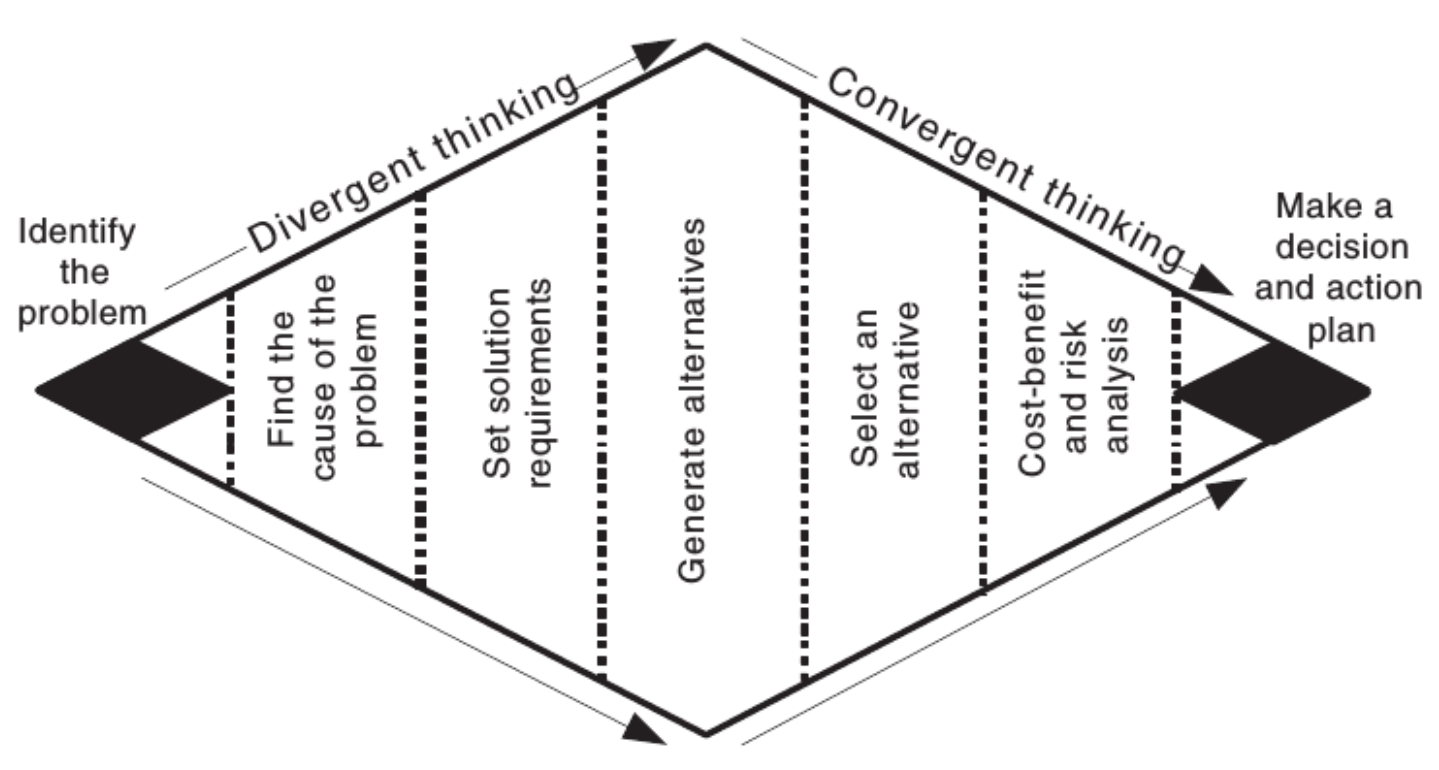
\includegraphics[width=0.8\textwidth]{taskAnalysis.png}
\end{center}

\paragraph*{Идентификация проблемы.} Нужно четко описать, в чём собственно проблема. На этом шаге уже могут возникнуть сложности. Проблема есть, все ее понимают, но когда начинаешь ковыряться в ней, оказывается что все понимают проблему по-разному, и в целом для разных людей разное является проблемой. Так что важно её явно проговорить, а можно куда-то и записать.

\paragraph*{Причина проблемы.} Нужно понять, что есть причина проблемы. Это может быть не всегда просто. Может потребоваться провести какой-то анализ, опросить людей, но нужно четко понять, что есть причина. Потому что именно ее нужно искоренить.

\paragraph*{Требование к получаемому решению.} Как будет хорошо? Что будет, когда будет хорошо? Что будет иначе?

\paragraph*{Генерация альтернатив.} На этом этапе часто бывают полезны мозговые штурмы и другие подходы к генерации идей. Это стадия, когда мы вширь начинаем строить дерево решений. 

\paragraph*{Выбор альтернативы.} Дальше идёт стадия, когда мы дерево решений начинаем сворачивать, отбрасывая альтернативы, и приходим к кому-то одному варианту.

\paragraph*{Оценка альтернативы.} Мы выбираем альтернативу, оцениваем её с точки зрения рисков, оцениваем её с точки зрения решения изначальной проблемы.

\paragraph*{План.} Стоим action-план: что нужно делать пошагово, чтобы решить проблему.

Бывают и более сложные фреймворки для принятия решения, но это отдельная большая область.

\subsection{Принятие решений}

Некоторые решения принимаются исключительно руководителем проекта, другие решения принимаются всей командой. Для того, чтобы это эффективно работало, необходимо понимание командой возможных способов решения проблемы и их сознательного выбора. Как принимаются решения и кем они принимаются, тоже очень важно для понимания.

Варианты принятия решения бывают следующие.

\paragraph*{Единогласный консенсус.} Все участники соглашаются единогласно с каким-то решением. Преимущества такого подхода: каждый проголосовал сам, все подписались под общим решением. Это говорит о том, что никто не против. Однако, если человек в команде много (хотя бы больше 10), то консенсуса достигнуть очень сложно: сколько людей, столько и мнений. Поэтому очень часто это все выливается в споры, убеждения друг друга, что может тянуться довольно долго. Если принимается очень важное решение и должен быть единогласный ответ, то необходимо наличие альтернативного плана (например, что если уже восемь часов прошло, а вы ещё не пришли к соглашению?).

\paragraph*{Голосование.} Это самая демократическая процедура, очень <<дешевый>>, быстрый способ, в который можно вовлечь много людей. В случае большого количества альтернативных решений можно провести несколько раундов голосований и прийти к итоговому решению. Но и все проблемы демократии тут тоже налицо: невежественное большинство может легко <<победить>> малочисленных, но разбирающихся в деле специалистов.

\paragraph*{Делегирование.} Передача решения небольшой группе специалистов, которая будет принимать решения от лица всей команды. Хороший пример~--- выбор базы данных разумно делать специалистам по базам данных. Вроде бы в таком подходе всё хорошо, но специалистам, которым делегировали задачу принятия решения, должны доверять все члены команды. Если такого доверия нет, то будет очень странно и опасно доверить принятие решения таким людям.

\paragraph*{Автократия.} <<Я послушаю ваши мнения, и сделаю так, как считаю нужным>>. Решения принимает лидер команды или менеджер, в зависимости от проблемы. Этот человек может делать это абсолютно самостоятельно, может на основе мнений команды/специалистов. При таком подходе нужно чтобы мнения всех членов команды были услышаны, иначе такое принятие решения будет не очень хорошим шагом, т.к. приведет к непониманию со стороны команды (вряд ли человек будет считать, что ему доверяют/уважают его мнение, если с ним не посоветовались). При такой системе человеку, который принимает решение, важно быть решительным, но при этом уметь прислушиваться к людям, т.к иначе можно очень легко потерять их доверие.

Важно, чтобы все члены команды чётко понимали, какие решение принимают каким образом.

\subsection{Разрешение конфликтов}

Возникновение конфликтов в команде неизбежно, поскольку принятие решений~--- творческий процесс. Опытные команды понимают важность конфликтов и умеют их решать. Это позволяет решить конфликт, достигнув наилучших результатов и при этом сохранив хорошие отношения.

Вариантов решения конфликтов очень много. Можно просто пытаться их избегать, например, введением правил или с помощью менеджера, который будет сразу же пресекать любые конфликты. Далее рассмотрим разные варианты решений конфликтов.

\paragraph*{Игнорирование.} Можно просто стараться не замечать конфликтов, попытавшись сконцентрироваться на хороших отношениях в команде. Однако, если конфликт серьезный, то это вряд ли приведет к чему-то хорошему, а лишь отсрочит неизбежное.

\paragraph*{Решение силой.} Можно попытаться навязать оппоненту своё решение силой, не думая о возможных последствиях (изменение отношений в коллективе и т.д.). Этот метод может подразумевать, в том числе, применение физической силы (повышение голоса и т.д.). Можно попытаться надавить с позиции авторитета, <<Я начальник, так что будет так, как я сказал>>. Хотя такой метод является весьма результативным, он всё же не является эффективным решением, поскольку его применение может резко ухудшить отношения в коллективе.

\paragraph*{Компромисс.} Принятие невыигрышного решения для обеих сторон конфликта. С одной стороны, такой подход выражает уважение сторон друг к другу, однако, это lose-lose стратегия, т.к. принимается решение, не удовлетворяющее ни одну из сторон. Поэтому такой подход тоже может оказаться неэффективным. Хорошее в этом подходе то, что столкновение явно выносится на обсуждение и разрешается лицом к лицу, в личном разговоре сторон. Суть данного метода заключается в решении конфликта, дабы избежать его нарастания. Однако при наличии профессионального конфликта такой конфликт лучше проанализировать и явно решить.

\paragraph*{Конфронтация конфликта.} Самый лучший вариант разрешения конфликта~--- это не давать им появляться. Например, введением аккуратных базовых правил, практик эффективного слушания, хорошо организованных совещаний и т.п. Но всё равно конфликты будут случаться, и тогда имеет смысл явно вынести его на обсуждение.

Первый шаг здесь~--- признание самого факта конфликта. Выскажите несогласие и проанализируйте эмоции, которые всплывают при конфликте. Обсуждение конфликта позволяет сконцентрироваться на проблеме, а не на людях. Вместо того, чтобы упорствовать и закапываться в позицию конфликта, каждая из сторон должна быть сфокусирована на своих целях, задачах и том, что хочется вынести из конфликта. Это позволяет взглянуть на конфликт в общем и начать движение в сторону решения, которое удовлетворит обе стороны. Часто помогает попытаться понять позицию противоположной стороны конфликта, причину, по которой возникло разногласие.

Для решения проблемы можно применять технику, описанную выше. Сфокусируйтесь на определении возможных решений, сгенерируйте большое количество возможных решений. Как и в случае с мозговым штурмом, такая тактика позволяет комбинировать идеи и расширить сознание команды.

Кроме того, должен быть вариант, когда стороны не могут договориться. Для такого случая должен быть запасной план, с привлечением третьей стороны для решения конфликта.

\section{Непрерывное обучение}

Непрерывное обучение подразумевает процесс постоянного развития команды, улучшение командной культуры, процесс анализа и обучения на предыдущих ошибках. Рассмотрим некоторые моменты, способствующие формированию такой среды непрерывного обучения.

\paragraph*{Создание культуры непрерывного обучения.} Высокоэффективные команды быстро развиваются, но это возможно лишь в условиях хорошо обозначенной культуры непрерывного обучения. Такой процесс вряд ли возможен в команде, где все новые и необычные идеи сразу же отклоняются, а любая ошибка жестоко порицается. Поэтому необходимо создать культуру, которая будет поддерживать и всячески поощрять непрерывное обучение и развитие членов команды в отдельности и самой команды в целом.

\paragraph*{Стремление к честности.} Многие люди избегают конфликтов, чтобы поддержать гармонию в проекте. Это не очень хорошо в том случае, когда замалчиваются/скрываются плохие новости или игнорируется информация, противоречащая планам проекта. Если реальные проблемы обсуждаются не на митинге, а после него, в коридорах, то это очень плохой знак. Кроме того, не стоит забывать, что люди могут просто бояться сказать о своих проблемах, а это может привести к очень плачевным последствиям. (Если вас заставят писать операционную систему на JS, а вы будете бояться сказать начальнику о том, что это~--- не лучшая идея, то из этого ничего хорошего не получится). Это плохой вариант развития для проекта. Чтобы быть эффективным, руководство должно всячески поощрять открытость внутри команды.

\paragraph*{Поощрение обучения.} Следует сделать обучение сознательной и постоянной целью команды. При разборе полетов во время митинга задавайте следующие вопросы: чему мы научились? что нам нужно изучить? какая информация позволит нам улучшить понимание задач, стоящих перед нами? Кроме того, следует начинать обсуждение проблемы не с предложения решений, а с задавания вопросов.

\paragraph*{Пересмотр целей и планов проекта.} Поскольку цели и план проекта были сформулированы в самом начале работы, то, вероятнее всего, прогресс в работе позволит взглянуть на них в новом свете. Кроме того, следует анализировать факты и допущения, которые привели к той ситуации, которая в данный момент образовалась в проекте. Поэтому периодически следует пересматривать цели, границы и план проекта. <<Если вы взбираетесь по лестнице, а потом понимаете, что она прислонена к не той стене, к которой должна была, то следует спуститься вниз и переставить лестницу>>.

\section{Особенности формирования команды}

Когда идет подбор персонала, часто встречается следующая ошибка: поиск максимально крутых специалистов. Если в команде есть две суперзвезды, то они, скорее всего, будут постоянно конфликтовать между собой. Это не зависит от конкретных людей, а просто является особенностью темперамента. Если есть человек, который чувствует себя техническим лидером в команде, то он, исполняя свою роль, просто поговорит со всеми и примет решение, поскольку он чувствует на себе ответственность за это. Если таких людей два или больше, то они будут конфликтовать по поводу того, чьё же решение должно быть принято, либо же будут перекладывать ответственность за принятие решений друг на друга (или на других людей), либо же просто подерутся и вообще никакого решения не примут. Поэтому очень плохо, когда в команде людей определенного типа больше, чем должно быть. Есть вполне четкие пропорции, которым должен соответствовать состав команды. Чаще всего, должна быть небольшая прослойка <<элиты>>, тех самых суперзвезд (альфа-самцов программирования). Но существование такой прослойки хоть и желательно, но вовсе не обязательно, её может и не быть. Должно быть небольшое количество новичков, но немного, иначе будет очень сложно укладываться в дедлайны. Новички в проекте нужны для передачи им знаний, компетенций, для обучения. Это некая гарантия развития проекта и передачи знаний о коде проекта. Основной частью проекта являются просто хорошие специалисты, которые пишут большую часть кода, делают основные задачи. Без такой прослойки продвижение проекта просто невозможно (иначе кто же будет делать работу?).

Кроме того, ни в коем случае нельзя забывать про необходимость наличия тестировщиков в команде. Сколько нужно тестировщиков на 10 программистов? Точного ответа на этот вопрос нет, но, как показывает практика, часто хватает одного тестировщика на трёх-четырёх программистов. Подходит ли вам это? Проверьте на практике, сделайте выводы. Вся команда должна понимать, что тестировщик~--- это правая рука всей команды. И если тестировщик нашёл баг в проекте, то мы не выпустим код в релиз, пока не исправим баг или не достигнем каких-то договоренностей с клиентом о том, что с этим багом делать. Как показывает практика, разработчики до конца свой код не проверяют. Конечно, написание модульных тестов немного решает проблему, но тестировщик всё равно необходим. Прежде всего потому, что это человек с особым складом ума, и он может найти такие баги, о которых команда разработчиков просто не подозревала.

Теперь о ролях и темпераменте в команде. Есть разные роли, каждая по-своему важна. Есть прирожденные лидеры, которые хотят славы, признания.

Есть технари, которым плевать на славу и признание, им просто нравится решать технические задачи. Они не хотят принимать решения, не хотят быть техническими лидерами, они просто хотят решать сложные задачи.

Есть люди, которые вообще работать не хотят, они просто могут быть душой компании, теми людьми, кто всё внутри команды организует. Парадокс, но такие люди тоже нужны. Казалось бы, что вместо такого человека можно взять более продуктивного человека, однако в ограниченном количестве такие люди всё же должны быть в команде. Это редко программисты (иначе это было бы слишком странно), чаще~--- HR’ы, офис-менеджеры, секретари и т.п. Такой человек может со всеми поговорить, расшевелить всех и т.д.

Не надо делать команду больше, чем надо. Казалось бы, чем больше программистов, тем лучше, но нет. Разные люди, разные темпераменты, разные компетенции, всё это очень трудно собрать воедино и заставить работать вместе, причем нужно не просто работать, а эффективно работать. Нельзя забывать об этом.

Не стоит забывать и про подходящее помещение. Всем должно быть комфортно работать, но при этом не слишком комфортно, чтобы всё-таки была работа, а не релаксация. Хорошо, если вся команда собрана в одном месте (угол большого офиса, например), поскольку это позволит избежать различных проблем с коммуникацией, которые могут возникнуть при сильно разбросанных территориально рабочих местах членов команды.

\subsection{Личные характеристики}

Все они так или иначе важны для подбора программистов. При подборе команды/нового человека нужно хотя бы бегло оценить все эти характеристики по списку:

\begin{itemize}
    \item Внутренняя/внешняя управляемость
    \item Высокая/низкая мотивация
    \item Умение быть точным
    \item Исполнительность
    \item Терпимость к неопределенности
    \item Эгоизм
    \item Степень увлеченности
    \item Склонность к риску
    \item Самооценка
    \item Личные отношения в коллективе
    \item ...
\end{itemize}

Рассмотрим теперь некоторые из пунктов чуть подробнее.

\paragraph*{Внутренняя/внешняя управляемость.} Это то, как человек относится к событиям, которые с ним происходят. То есть, сам человек управляет событиями, или же события управляют им. Нужно понимать, к какому из этих типов относится человек, которого вы принимаете к себе в команду, дабы в дальнейшем избежать непонятных ситуаций.

\paragraph*{Высокая/низкая мотивация.} Тут всё вполне понятно: личности с высокой степенью мотивации способны разрабатывать очень сложные и сравнительно надежные программы, а личности с низкой степенью мотивации чаще всего не хотят ничего делать (не будут работать, пока их не пнёшь). Руководители, способные повысить уровень мотивации, в то же время, могут стимулировать своих сотрудников к созданию программ с высоким уровнем безопасности.

\paragraph*{Умение быть точным.} Характеристика, которая для программиста очень важна. Если программист не способен быть точным и внимательным, он будет постоянно допускать ошибки из-за невнимательности. Если всё-таки есть такой человек в команде, то его код нужно просто постоянно ревьюить и проверять на наличие ошибок.

\paragraph*{Терпимость к неопределенности.} Показывает то, насколько человек способен терпеть неопределенность. Насколько человеку нужно то, чтобы все было четко и понятно? Чаще всего постоянно идет борьба с неопределенностью. Есть люди, у которых от неопределенности постоянный стресс. В зависимости от этого фактора человека просто нужно распределять на разные задания.

Все эти качества нужно так или иначе оценивать на собеседовании. Это приходит с опытом, нужно уметь подбирать себе команду.

\section{Командная разработка}

Если говорить про программирование, то командная разработка очень сильно отличается от разработки проектов в одиночку. Нужен единый стиль оформления (чтобы, скажем, никто не подрался из-за вечного холивара <<табы или пробелы>>), больше тестов, больше документации. Нужно организовать процесс ревью кода, коллективных ревью. Если в проекте используются различные third-party библиотеки, то нужно договориться о том, какую версию вся команда будет использовать, иначе будет полный хаос. Ну и командная разработка вряд ли возможна без системы контроля версий.

\end{document}
